\part{Présentation des résultats}
\chapter{}
\section{Presentation}
Les données brutes sur lesquelles se portent  mes résultats se trouvent sur mon  \href{https://github.com/the0phil3/projetMemoire/}{Github} dans le fichier tsv \emph{'mortsduRif'}. Grâce à la quantité de données dont j’ai disposé, j’ai pu procéder à plusieurs manipulations afin d' apporter des explications sur ce qui s’est passé pendant la guerre. La logique qui m’a guidé dans  mes extrapolations a consisté à essayer de pallier au manque de données chiffrées présentées par Max Schiavon dans son ouvrage sur la guerre des français au Rif. Je fais référence à un tableau qu’il y a inclus  indiquant le nombre de morts dûs à  la guerre pendant l’offensive rifaine, entre le printemps et une partie de l’été 1925 : 
\begin{figure}[H]
    \centering
    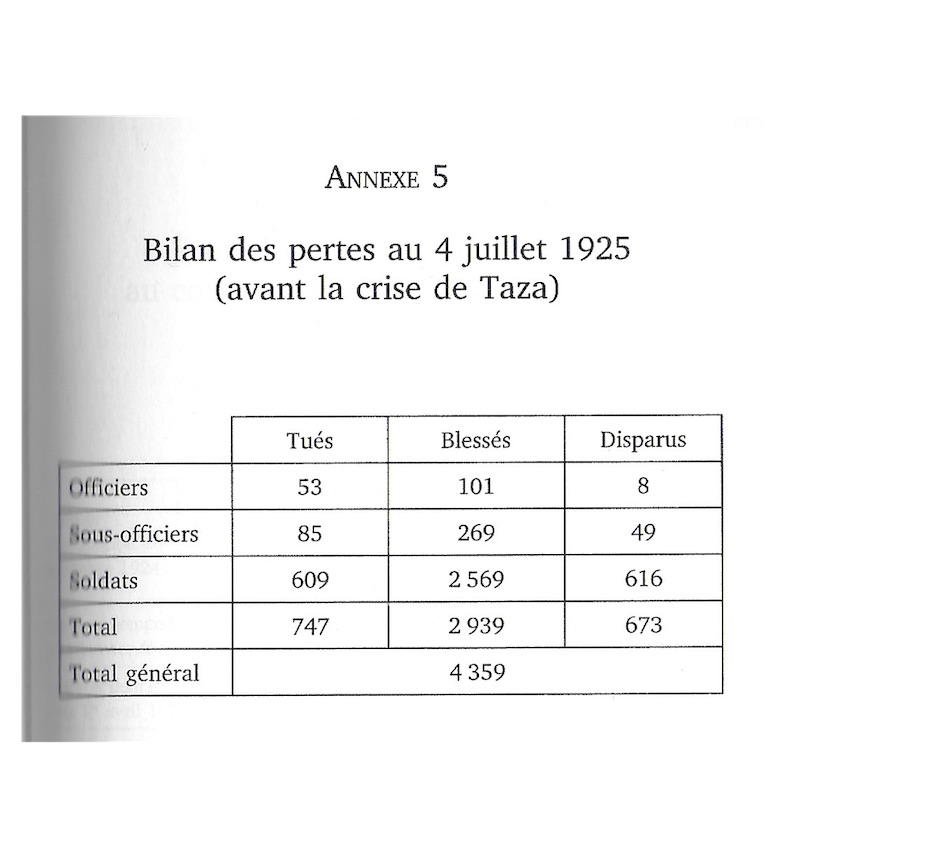
\includegraphics[scale=0.36]{Images/schiavon.jpeg}
    \caption[Note d'image]{Données de Schiavon indiquant les morts avant le 4 juillet 1925\footnotemark}
    \label{fig:Morts Schiavon }
\end{figure} 
\footnotetext{\footcites[309]{schiavon2016}} 
A première vue, il semble que nos données ne coïncident pas  : Schiavon n'enregistre que 747 morts pour les 6 premiers mois de la guerre alors que mes données indiquent 4679 morts pour les deux années de combat. Pourtant, lorsque nous l’on examine en profondeur les dates clés de la guerre et les chiffres fournis par Schiavon et qu’on les compare avec les témoignages des officiers, on constate  que, bien que l'on ne sache pas exactement où Schiavon a recueilli ses données, les deux sont à priori cohérents. Mes résultats se concentrent sur trois domaines
: \begin{enumerate}
    \item les dates
    \item les lieux 
    \item les régiments
\end{enumerate} 

\section{Les dates}
En filtrant pour les dates de la guerre durant lesquelles il y a eu le plus de pertes françaises, j’ai cherché à établir une chronologie des pertes afin de les comparer avec l’historiographie et toute éventuelle informations que les JMOs ou registres matricules pourraient apporter. Les résultats que j’ai obtenus en calculant les jours où il y a eu  le plus de pertes sont présentés dans la figure 3.2. Ce qui est frappant dans cette figure est la prédominance de la période 1925 à 1926 dans son caractère meurtrier. Cette tendance est commune au reste des résultats pour les dates, qui se trouvent en annexe.\footnote{Voir annexe : \ref{fig:Dates 2}}
\begin{figure}[H]
    \centering
    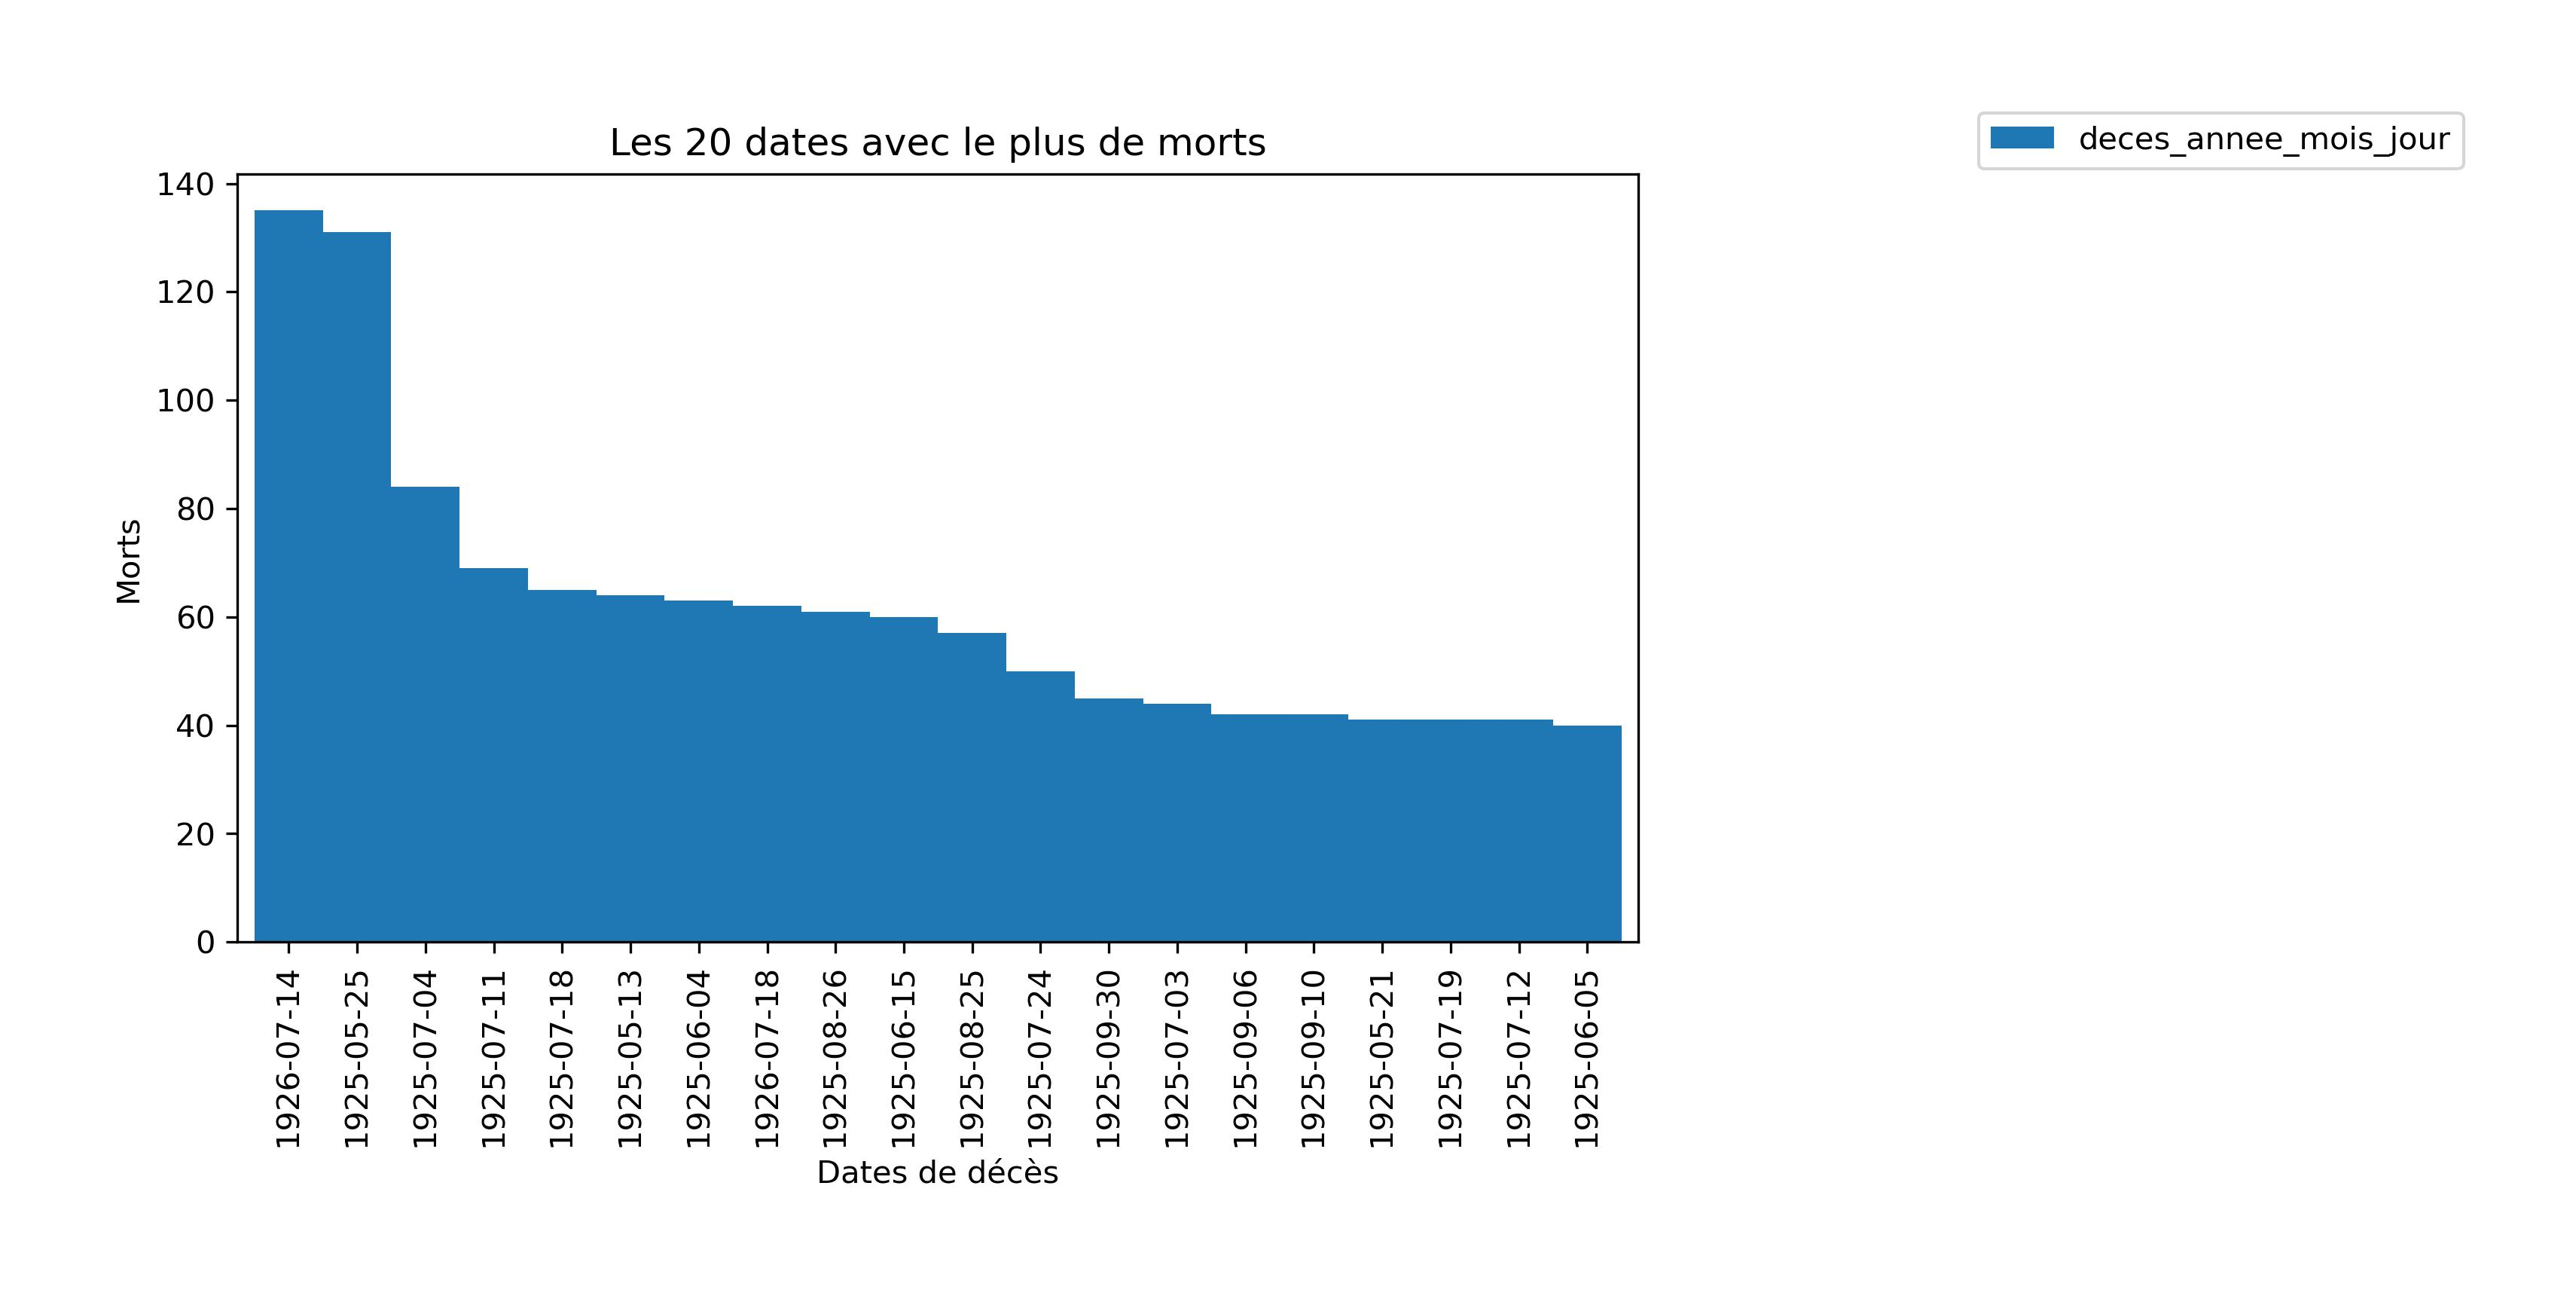
\includegraphics[scale=0.58]{Images/20dates.jpg}
    \caption{Les 20 jours avec le plus de pertes pour l'armée française}
    \label{fig:Morts par jour}
\end{figure}
En outre, la date qui enregistre le plus grand nombre de morts, le 14 juillet 1926, est curieuse car il s’agit d’ une valeur isolée dans la tendance. Lorsqu’on examine les récits de l’offensive française de 1926, on comprend pourquoi cette journée a été si meurtrière. Dans le témoignage du jeune lieutenant Joubert, la préface du général Dufieux décrit l’attaque de « la grande Tache de Taza » où l’avant-garde de la brigade de Ganay sous le commandant Croizé résiste  aux Rifains.\footcites[7]{joubert1927} Le commandant Croizé meurt quatre jours plus tard lors de la même offensive. Par ailleurs, si l’on essaie  de situer mes données dans la chronologie de Schiavon, on comprend pourquoi son tableau contient si peu de morts. Il correspond à des dates antérieures à la fin de la période dite " Héroïque " de la guerre lorsque l'armée française n'est pas encore sollicitée jusqu'au point de rupture.\footcites[143]{schiavon2016}La lecture que fait Schiavon de ses propres données est révélatrice pour mon comparatif car il présente lui-même leurs propres insuffisances. Il écrit qu’ à ces chiffres de 1 005 morts, il faut ajouter 997 disparus et 478 morts par maladie, accident ou suicide, ce qui porte le décompte à environ 2 480 morts.\footcites[145]{schiavon2016} Un chiffre qui correspond mieux aux relevés du SHD compilés 100 ans après ce conflit. .
\section{Les lieux}
Les informations que la base de données de morts fournit pour les lieux de décès sont également en accord avec les  tendances historiographiques de la guerre du Rif. La figure 3.3 donne un aperçu de mes résultats pour le calcul des lieux avec le plus de pertes. Le reste de figures se trouvent dans les annexes.\begin{figure}[H]
    \centering
    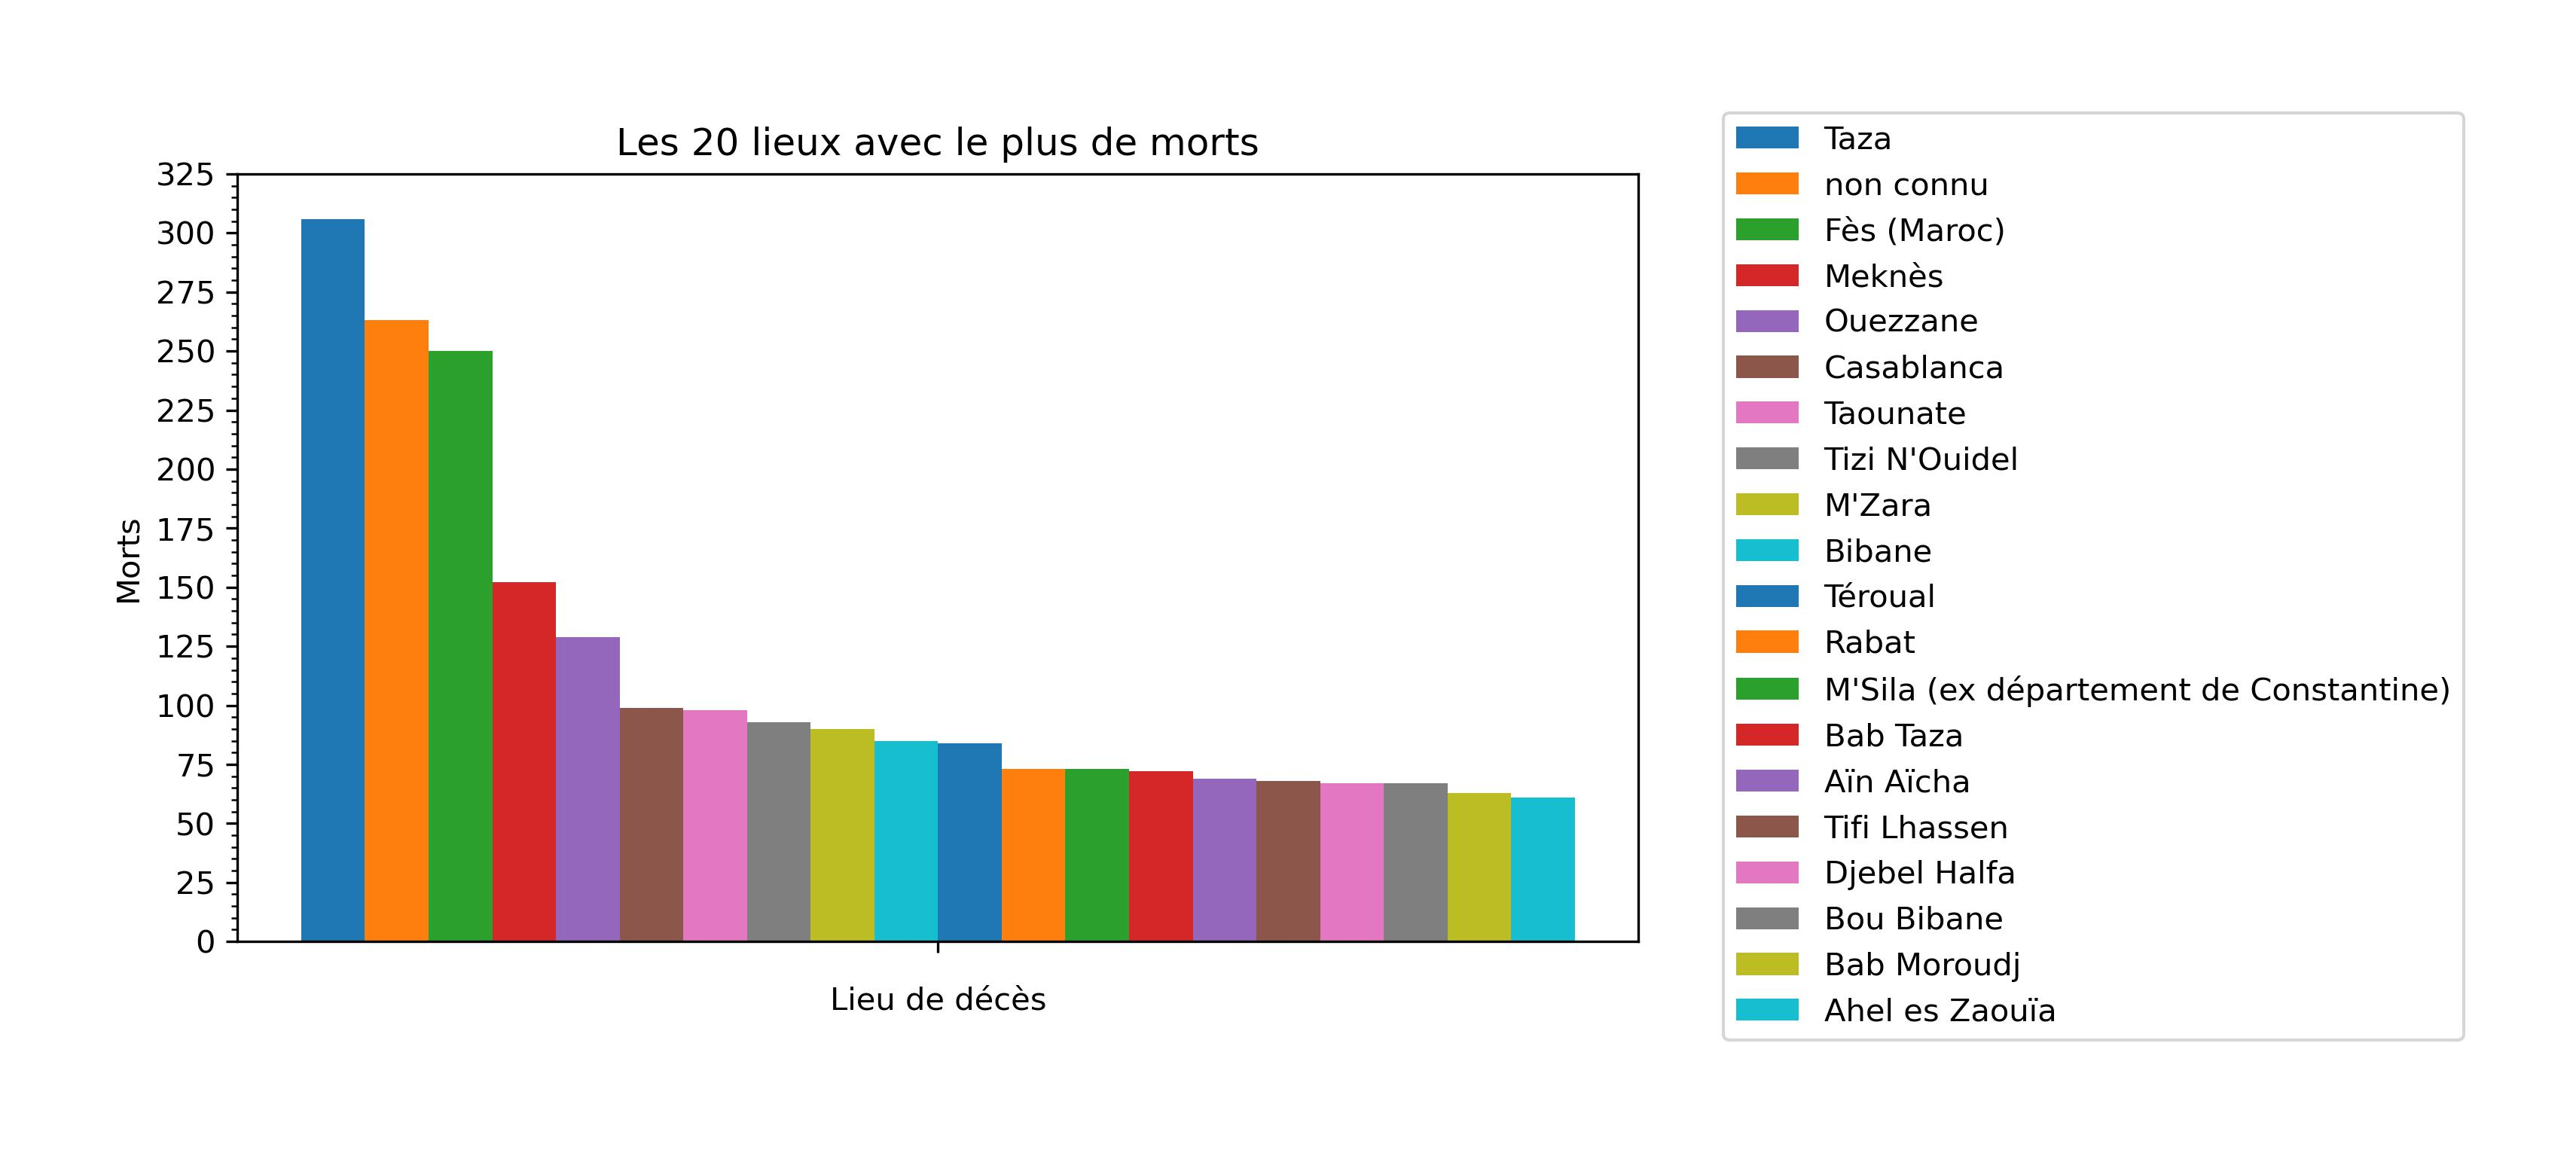
\includegraphics[scale=0.5]{Images/20places.jpg}
    \caption{Les 20 lieux avec le plus de pertes pour l'armée française}
    \label{fig:Morts par lieux}
\end{figure} 
La prédominance de lieux comme Taza, Ouezzane et Meknès dans la partie supérieure de la figure correspond précisément aux récits dominants du conflit. Le témoignage de Walter B. Harris, spécialiste du Maroc, contemporain de la guerre, indique que les combats les plus violents de la campagne de 1925 ont eu lieu sur la ligne entre Taza et Ouezzane.\footcites[226]{harris1925} L’analyse de Schiavon est tout à fait en accord avec ce constat. 
\section{Les régiments}
En ce qui concerne les régiments qui ont subi le plus de pertes, la question de la conformité des résultats à l'état actuel de l'historiographie est plus complexe. Ceci est dû au manque d’études sur le sujet. En dehors de  Schiavon, qui soutient que les soldats métropolitains et officiers subalternes ont subi une plus grande proportion de pertes dans leurs effectifs que les soldats nord-africains, très peu d’études ont été consacrées aux différentes composantes des armées français qui y ont participé.\footcites[145]{schiavon2016} D'après mes résultats, on peut constater que les régiments de la légion étrangère composés de soldats non-français mais non issus l’empire, ont un place importante. Mais les différents régiments de tirailleurs occupent aussi une place de choix en haut du classement.
\begin{figure}[H]
    \centering
    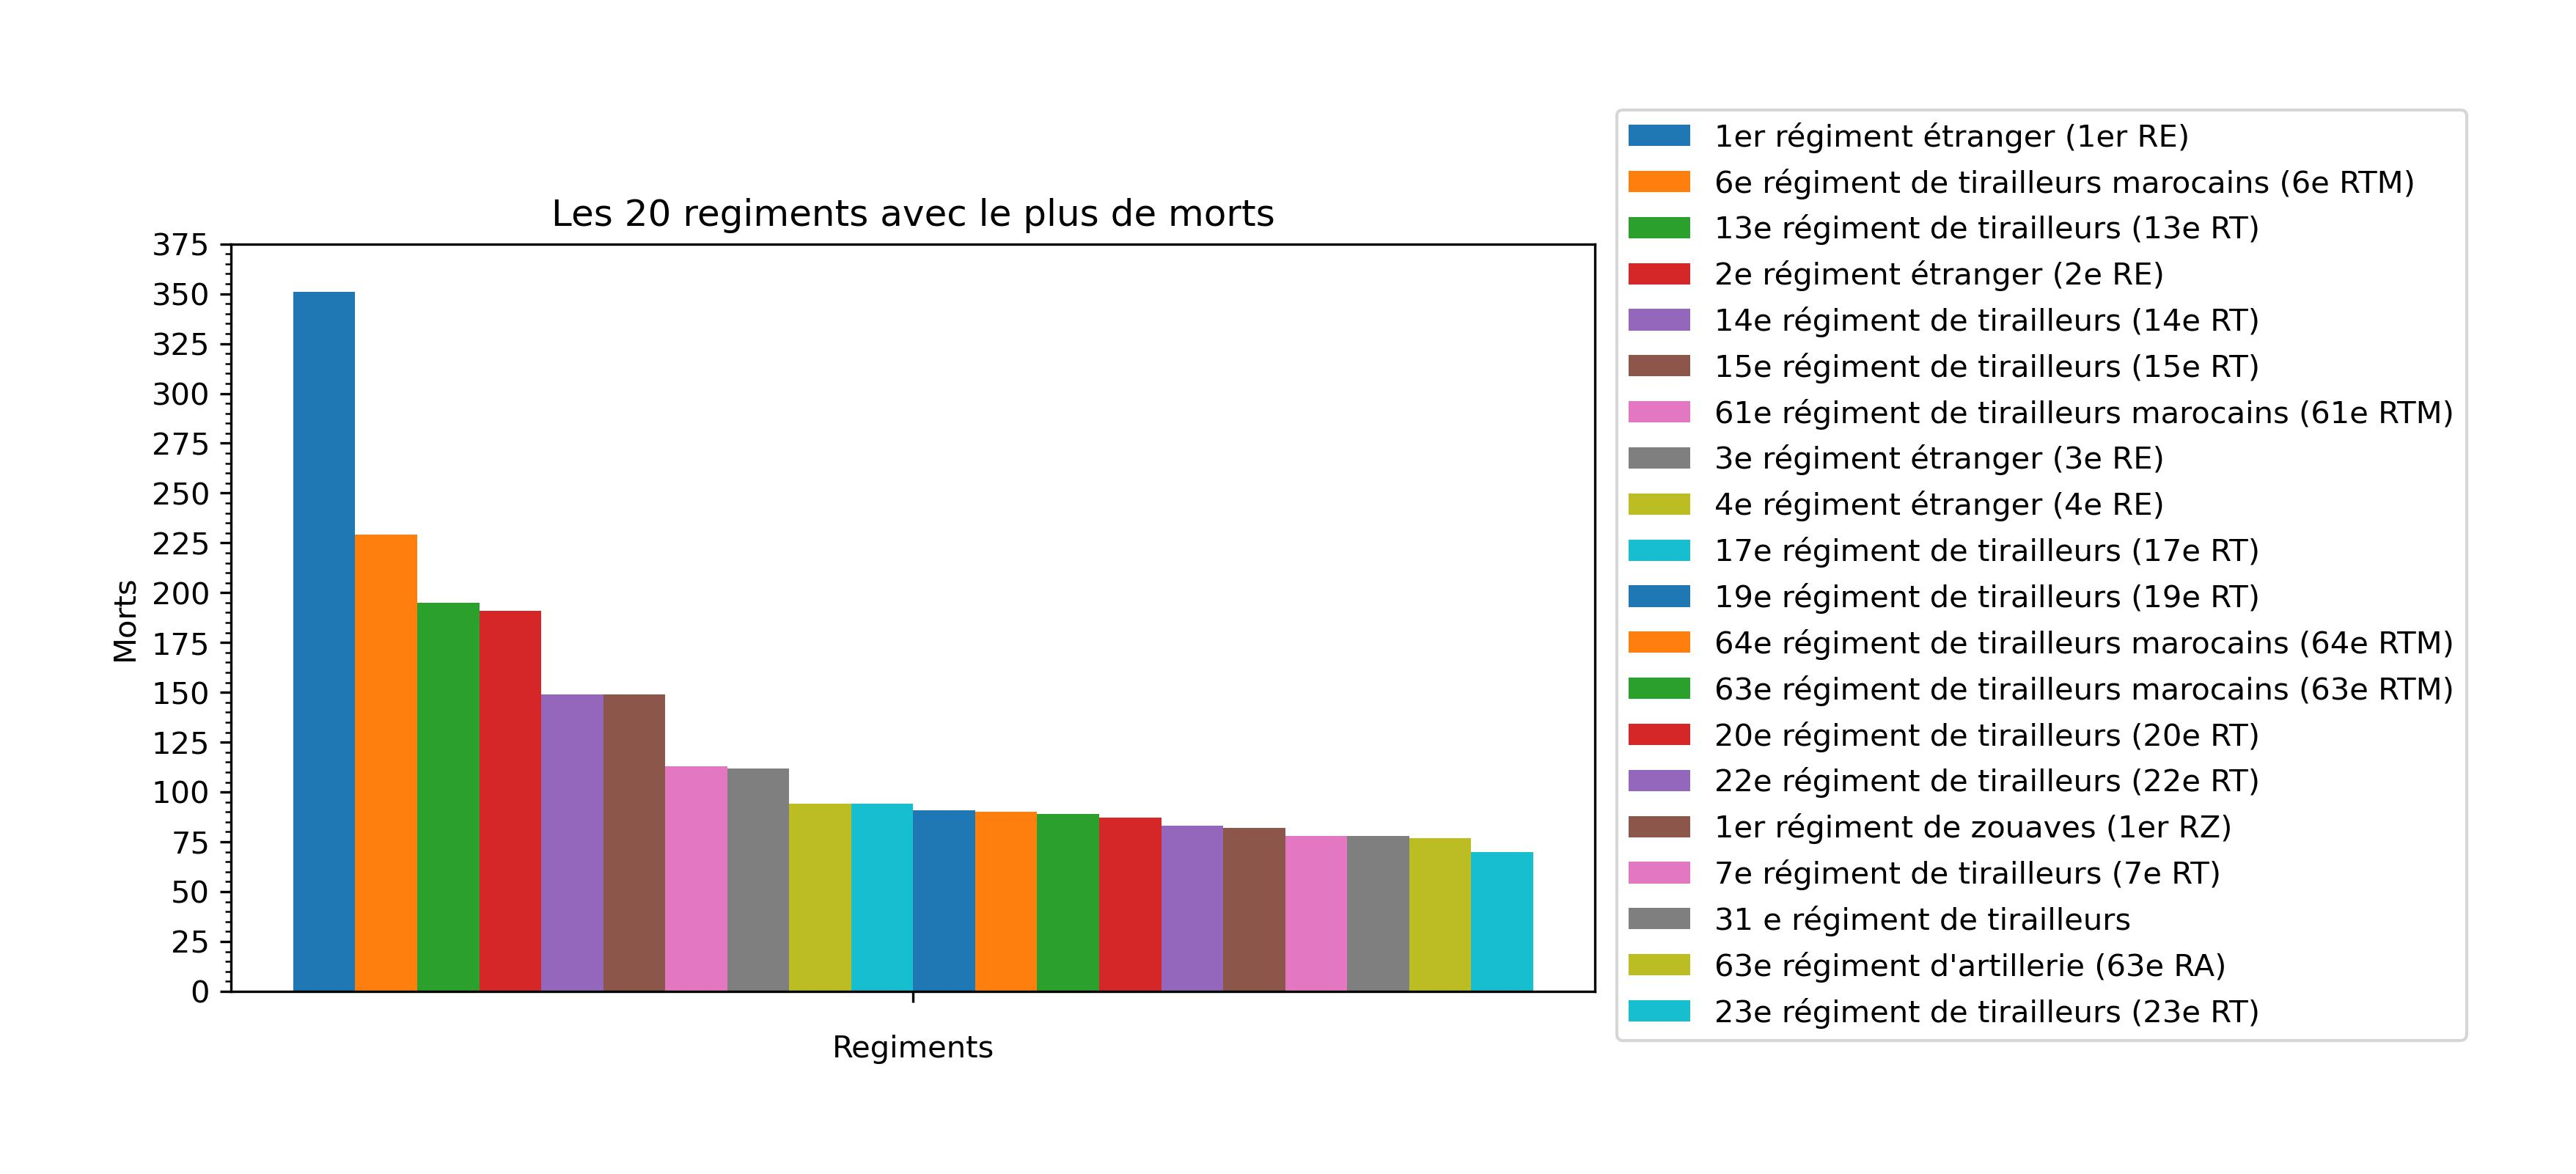
\includegraphics[scale=0.6]{Images/20regiments.jpg}
    \caption{Les 20 régiments avec le plus de pertes pour l'armée française}
    \label{fig:Morts par régiments}
\end{figure} 
 En observant l’ensemble des figures jointes dans l'annexe, il est clair que les régiments nord-africains sont majoritairement représentés dans les régiments ayant subi les plus pertes. Une explication potentielle de la présence des régiments de la légion en haut du classement des pertes pourrait venir de leur réputation de troupes d’élites. Dans l’ensemble, ces résultats restent difficiles à expliquer et contextualiser sans une idée claire du nombre de troupes préparées pour la campagne par régiment. Cette information pourrait se trouver dans les JMOs.

\section{Conclusion}
Bien que certains éléments importants manquent, l’ensemble de mes résultats sont en accord avec le faible éclairage  historiographique existant. Cependant, le résultat est un indicateur positif de la qualité des données disponibles sur le SHD. Cela ne signifie pas pour autant que d'autres travaux historiques doivent être négligés ou que ma méthodologie ne doit pas être remise en question. La taille  de la base de données montre clairement qu'il y a beaucoup plus de latitude pour analyser, comparer et traiter les caractéristiques des soldats qui y sont enregistrés.   
